\documentclass[12pt]{article}%
\usepackage{amsfonts}
\usepackage{fancyhdr}
\usepackage{comment}
\usepackage[letterpaper, top=2.5cm, bottom=2.5cm, left=2.2cm, right=2.2cm]%
{geometry}
\usepackage{times}
\usepackage{amsmath}
\usepackage{changepage}
\usepackage{multirow}
\usepackage{amssymb}
\usepackage{tikz}
\usetikzlibrary{arrows.meta}
\usepackage{graphicx}%
\graphicspath{ {images/} }
\usepackage{amsmath}
\setcounter{MaxMatrixCols}{30}
\newtheorem{theorem}{Theorem}
\newtheorem{acknowledgement}[theorem]{Acknowledgement}
\newtheorem{algorithm}[theorem]{Algorithm}
\newtheorem{axiom}{Axiom}
\newtheorem{case}[theorem]{Case}
\newtheorem{claim}[theorem]{Claim}
\newtheorem{conclusion}[theorem]{Conclusion}
\newtheorem{condition}[theorem]{Condition}
\newtheorem{conjecture}[theorem]{Conjecture}
\newtheorem{corollary}[theorem]{Corollary}
\newtheorem{criterion}[theorem]{Criterion}
\newtheorem{definition}[theorem]{Definition}
\newtheorem{example}[theorem]{Example}
\newtheorem{exercise}[theorem]{Exercise}
\newtheorem{lemma}[theorem]{Lemma}
\newtheorem{notation}[theorem]{Notation}
\newtheorem{problem}[theorem]{Problem}
\newtheorem{proposition}[theorem]{Proposition}
\newtheorem{remark}[theorem]{Remark}
\newtheorem{solution}[theorem]{Solution}
\newtheorem{summary}[theorem]{Summary}
\newenvironment{proof}[1][Proof]{\textbf{#1.} }{\ \rule{0.5em}{0.5em}}

\newcommand{\Q}{\mathbb{Q}}
\newcommand{\R}{\mathbb{R}}
\newcommand{\C}{\mathbb{C}}
\newcommand{\Z}{\mathbb{Z}}

\newcommand*{\pd}[3][]{\ensuremath{\frac{\partial^{#1} #2}{\partial #3}}}

\usepackage{enumerate}% http://ctan.org/pkg/enumerate
\usepackage{array}% http://ctan.org/pkg/array
\newcolumntype{M}{>{$}c<{$}}


\begin{document}

\title{CS 440/ECE448 Homework 6}
\author{Tanishq Dubey (tdubey3)}
\date{\today}
\maketitle
\section*{Problem 1}
    \begin{enumerate}[a)]
        \item
            \textbf{Over-fitting}: When a statistical model represents noise, or unwanted information. This usually happens when our model has unwanted information, has too much information, or is too small.
        \item
            There are two methods that can be used to prune a decision tree:
            \begin{enumerate}[1.]
                \item \textbf{Reduced Error Pruning}: This method starts at the bottom of the tree and moves upwards. At each node, a algorithm decides which side (class) is most popular and removes the others. If this change does not change the accuracy of the tree for the worse, the change is kept. This method traverses the entire tree.
                 \item \textbf{Cost Complexity Pruning}: This method generates a series of trees, where each tree has a reduced number of sub-trees (essentially, pre-pruned) and the final tree is just the root. Next, each sub-tree is tested for error. The sub-tree that has the most error is removed. After all trees have been generated, the one with the least error is kept as the final pruned tree.
            \end{enumerate}
        \item
            Pruning helps address the problem of over-fitting by removing sub-trees that do not contribute to the decision tree, but instead only add complexity and noise.
        \item
            Since pruning is used to address the problem of over-fitting, the alternatives to pruning must also address the same problems. One such method is to reduce the various parameters of the decision tree, thus artificially reducing the chance of over-fitting. This includes limiting depth, height, or even the number of tests performed on the tree. Another method is to estimate parameters to try and make a optimal tree, but this should be combined with limiting the tree.
    \end{enumerate}

\section*{Problem 2}
    \[n = \frac{k^{h+1} -1}{k -1}\]
    \[L = k^h\]
    \[h = log_kh\]
    \[n_{min} = \frac{k^{h+1} -1}{k -1} - L\]
    \[n_{min} = \frac{k^{log_k L+1} -1}{k -1} - L\]
    Thus:
    \[n_{min} = \frac{kL -1}{k -1} - L\]
\section*{Problem 3}
    \begin{enumerate}[a.]
        \item 
        To calculate entropy, of a single attribute, the following formula can be employed:
            \[E(s) = \sum\limits_{i=1}^{c} -p_ilog_2p_i\]
        Where, $C$ is the attribute we wish to find the entropy of.
        In our case, we only wish to find the entropy of the entire set of data. Thus we can calculate this value as such: 
            \[-\frac{200}{400}log_2(\frac{200}{400}) - \frac{200}{400}log_2(\frac{200}{400}) = 1\]
        \item
        To see information gain, the entropy of the various types of player abilities. With this we get the following sets of data:
        \begin{center}
            \begin{tabular}{c|c|c}
                Male Player Strength & Play Together Count & Not Play Together Count\\ \hline \hline
                Smash & 100 & 100\\ \hline
                Drop & 100 & 100\\ \hline
            \end{tabular}
        
            \begin{tabular}{c|c|c}
                Female Player Strength & Play Together Count & Not Play Together Count\\ \hline \hline
                Smash & 100 & 100\\ \hline
                Drop & 100 & 100\\ \hline
            \end{tabular}
        
            \begin{tabular}{c|c|c}
                Same Handedness & Play Together Count & Not Play Together Count\\ \hline \hline
                YES & 70 & 140\\ \hline
                NO & 130 & 60\\ \hline
            \end{tabular}
        \end{center}
        We can then calculate entropies for each attribute:\\
        \textbf{Male Player Strength:}
        \[E(Play Count, Male Player Strength) = P(Smash)*E(100,100) + P(Drop)*E(100,100)\]
        \[= (.5 * -\frac{100}{200}log_2(\frac{100}{200}) - \frac{100}{200}log_2(\frac{100}{200})) + (.5 * -\frac{100}{200}log_2(\frac{100}{200}) - \frac{100}{200}log_2(\frac{100}{200}))\]
        \[ = .5 * 1 + .5 * 1\]
        \[ = 1\]
        \textbf{Female Player Strength}
        \[E(Play Count, Female Player Strength) = P(Smash)*E(100,100) + P(Drop)*E(100,100)\]
        \[= (.5 * -\frac{100}{200}log_2(\frac{100}{200}) - \frac{100}{200}log_2(\frac{100}{200})) + (.5 * -\frac{100}{200}log_2(\frac{100}{200}) - \frac{100}{200}log_2(\frac{100}{200}))\]
        \[ = .5 * 1 + .5 * 1\]
        \[ = 1\]
        \textbf{Same Handedness}
        \[E(Play Count, Same Handedness) = P(YES)*E(70,140) + P(NO)*E(130,60)\]
        \[= (.525 * -\frac{70}{210}log_2(\frac{70}{210}) - \frac{140}{210}log_2(\frac{140}{210})) + (.475 * -\frac{130}{190}log_2(\frac{130}{190}) - \frac{60}{190}log_2(\frac{60}{190}))\]
        \[ = .525 * .9183 + .475 * .8997\]
        \[ = .9094\]
        Thus the information gain for the three split categories is:
        \begin{center}
            \begin{tabular}{c|c}
                Split & Information Gain \\ \hline \hline
                Male Player Strength & 0 \\ \hline
                Female Player Strength & 0 \\ \hline
                Same Handedness & .0905\\ \hline
            \end{tabular}
        \end{center}
        Based on this data, "Same Handedness" would be the root of the tree as per the ID3 algorithm.
        \item
        As stated in problem 2, the minimum number of nodes needed for a k-ary decision tree with L distinct classes is:
        \[n_{min} = \frac{kL -1}{k -1} - L\]
        Using this formula with $k=2$ and $L=8$, we get:
        \[n_{min} = \frac{16 -1}{1} - 8\]
        \[n_{min} = 12\]
        Using the generic height of tree formula - $log_2N$, with $N$ being the number of nodes - we can get:
        \begin{multline*}
        log_2(12) = 3.58496250072115618145373894394781650875981440\\
        7692481060455752654541098227794358562522280474\\
        9180882420909806624750591673437175524410609248\\
        2214208395062169829949365759223858523444158253\\
        6302747685306978051687599554473726683462461236\\
        4248850047581810676961316404807130823233281262\\
        4452486706338980148372342357836624783901189770\\
        0646631263422336334182127010609804917747254135\\
        7330110499026268818... \approx 3
        \end{multline*}
        Thus the height of our tree is 3.
        \item
        If we have a tree limited to a height of one, then to calculate the error of the tree, we simply compare what we expected to come out in our tree, to what we actually obtain. After parsing this tree, we can see that our error is 32.5\%. This is because we use the equation
            \[Error = \frac{Observed - Expected}{Expected}\]
        to find the error. Our observed value is the value of how many people played together when they should have, while our expected is as stated.
        \item
        Simply by looking at the data, it can be seen that a simple sorting algorithm for this data is seeing if the players have opposite attributes. By picking this split, we get 100\% accuracy for our data with a tree that looks like such:
        \begin{center}
            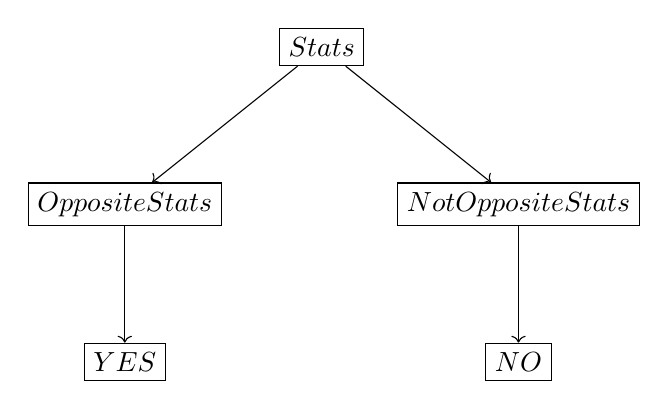
\begin{tikzpicture}
                \node[shape=rectangle,draw=black] (A) at (5,2) {$Stats$};
                \node[shape=rectangle,draw=black] (B) at (2.5,0) {$Opposite Stats$};
                \node[shape=rectangle,draw=black] (C) at (7.5,0) {$Not Opposite Stats$};
                \node[shape=rectangle,draw=black] (D) at (2.5, -2) {$YES$};
                \node[shape=rectangle,draw=black] (E) at (7.5,-2) {$NO$};

                \path [->](A) edge node[left] {} (B);
                \path [->](A) edge node[left] {} (C);
                \path [->](B) edge node[left] {} (D);
                \path [->](C) edge node[left] {} (E);
            \end{tikzpicture}
        \end{center}
        \item
        This tree has a height of 2, which is smaller than the ID3 tree because it is based off of patterns that a human can see but the ID3 algorithm cannot. In this case then, the smaller tree corresponds to the more accurate version
        \item
        As previously stated, the ID3 will not produce a globally optimal solution because it cannot see all the patterns present in the data, and thus cannot build a globally perfect tree.
    \end{enumerate}
\end{document}